% **************************************************************************** %
%                                                                              %
%                                                     ::::::::  :::::::::      %
%    sec_intro.tex                                      :+:      :+:    :+:    %
%                                                    +:+        +:+    +:+     %
%    By: A. Campo <andoitzcp@gmail.com>              +#+        +#++:++#+      %
%                                                    +#+        +#+            %
%    Created: 2022/11/18 22:55:54 by A. Campo        #+#    #+# #+#            %
%    Updated: 2023/02/09 08:22:25 by acampo-p         ###   ########.fr        %
%                                                                              %
% **************************************************************************** %

\section{INTRODUCCIÓN}

El sector de la automoción,
engloba una gran variedad de industria y servicios dedicados a servirla.
Se estima que la aportación económica total de las actividades relacionadas,
en este sector, asciende a un 11\% del PIB,
lo que la convierte en la industria manufacturera que mas ingresos aporta
después  del 18,8\% del PIB que posee la industria agroalimentaria española
(Díaz y Montorriol Garriga, 2021).
Esta cifra puede ser contrastada
frente a la carta emitida por el presidente de la ANFAC,
adherida al informe anual,
donde se aprecian estimaciones similares.

En este sector, el vehículo de propulsión autónoma,
es generalmente utilizado tanto por los servicios de transporte a pasajero,
como por los servicios logísticos dedicados al transporte de mercancías.
Entre los componentes que forman el vehículo autónomo,
se encuentran las cubiertas o neumáticos,
los cuales se comportan como enlace entre el vehículo y el pavimento.
Este nexo permite una transmisión eficiente
de la energía producida por el motor de combustión interna,
y a su vez, sus propiedades elásticas atenúan las irregularidades de la vía.

La industria manufacturera de cubiertas,
ha mantenido un incremento sostenido en su producción en los últimos años,
como puede observarse en la Figura \ref{fig:1_global_prod_evo}.
El mercado de neumáticos es liderado por dos empresas: Bridgestone y Michelin
\citep{rodgers2020tire}.
Las demás empresas compiten entre ellas
a un magnitud inferior a los lideres del sector,
como se aprecia en la Figura \ref{fig:1_brand_revenue}.

\begin{figure}[h]
	\begin{center}
		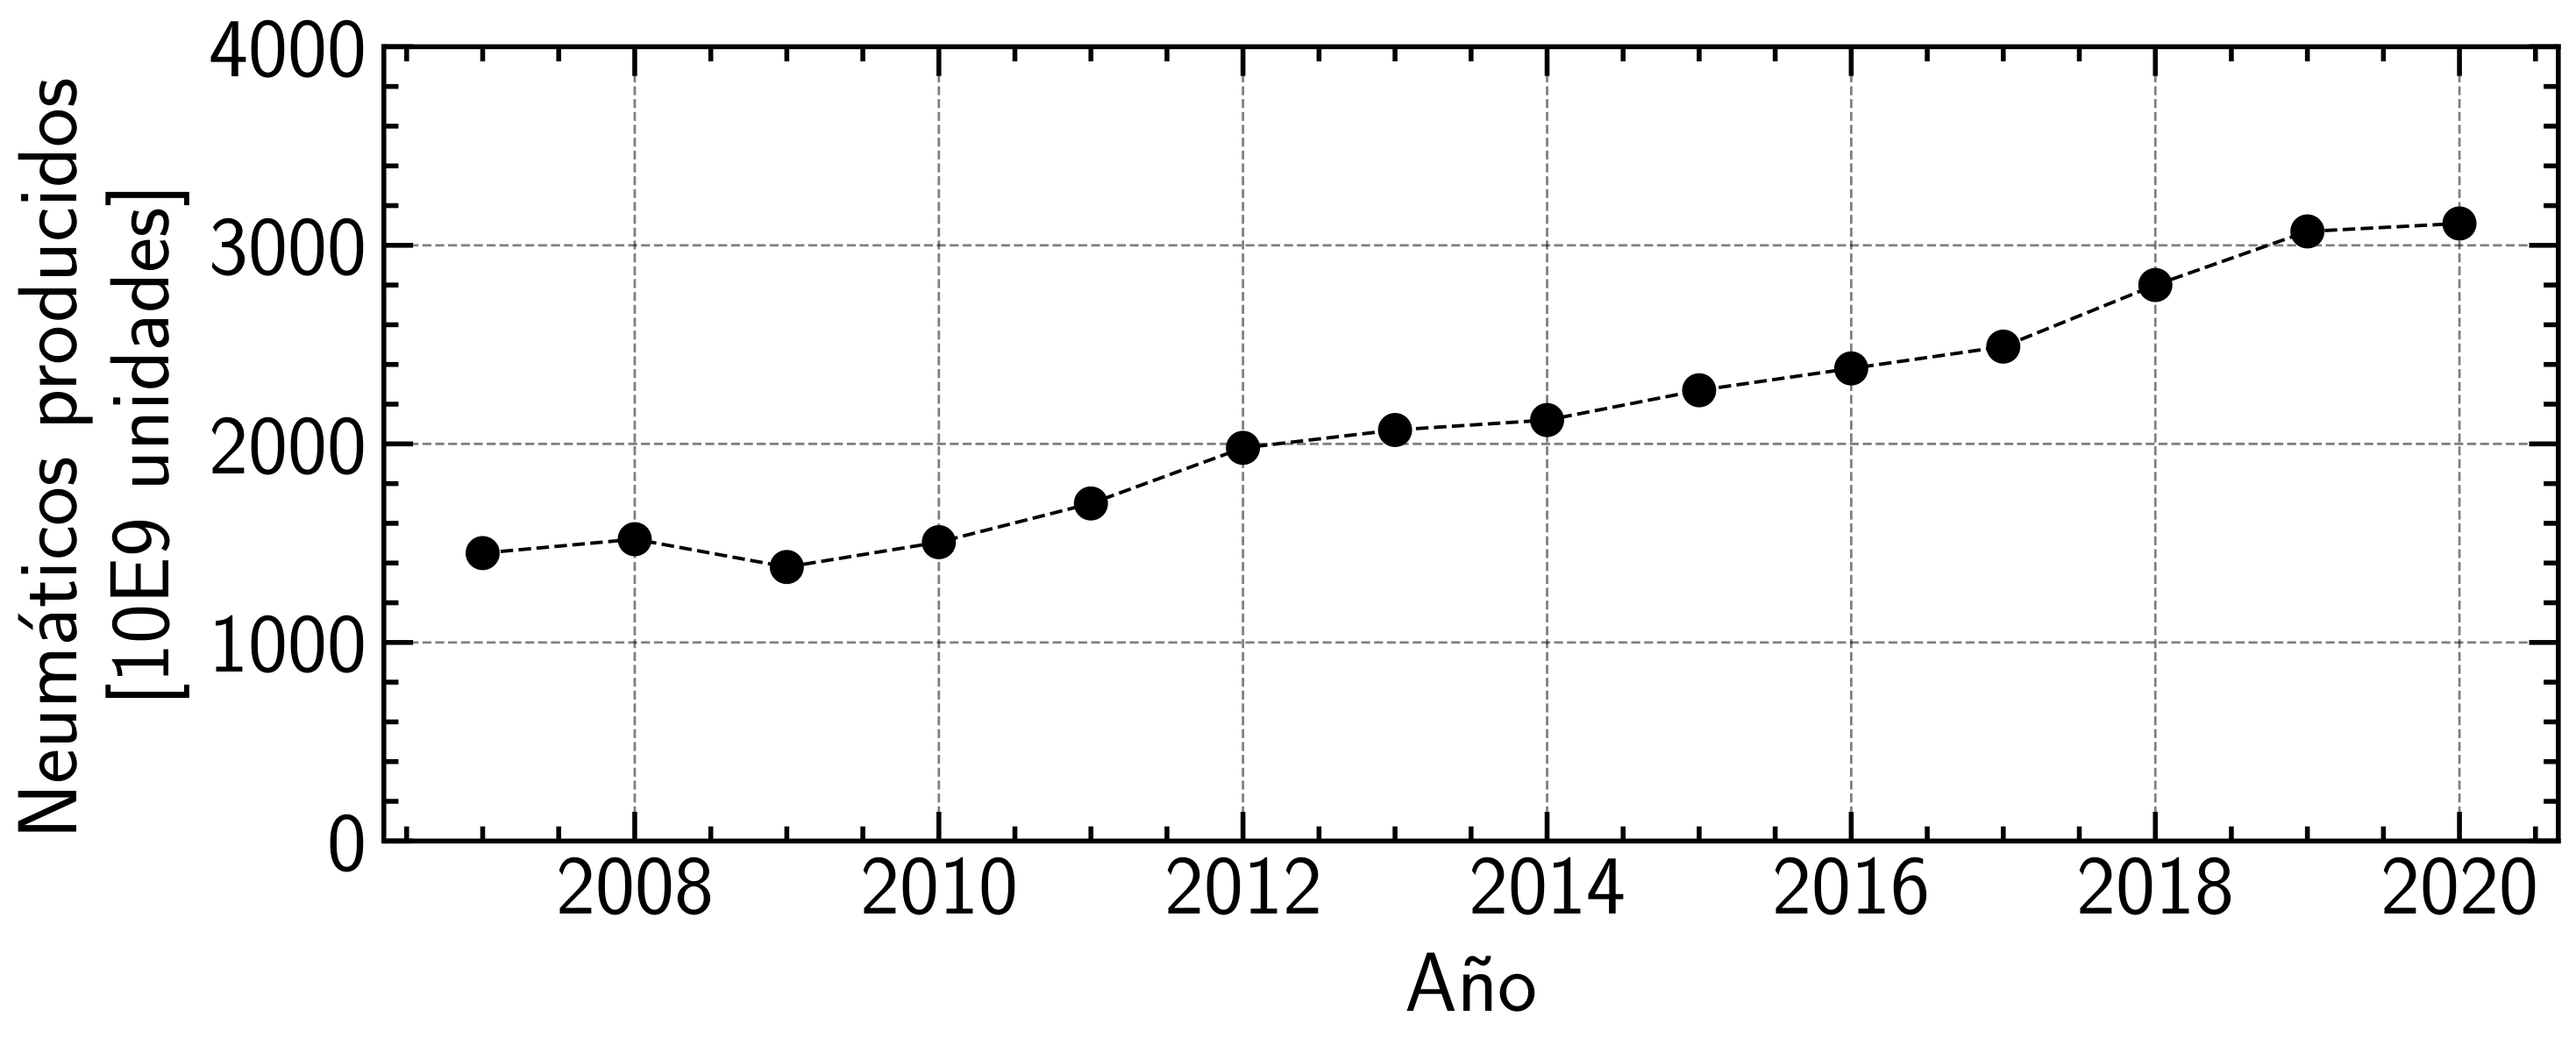
\includegraphics[width=\textwidth]{fig/1_global_prod_evo.PNG}
	\end{center}
	\caption{Evolución de la producción mundial de cubiertas.}
	\label{fig:1_global_prod_evo}
\end{figure}

 \begin{figure}[h]
	\begin{center}
		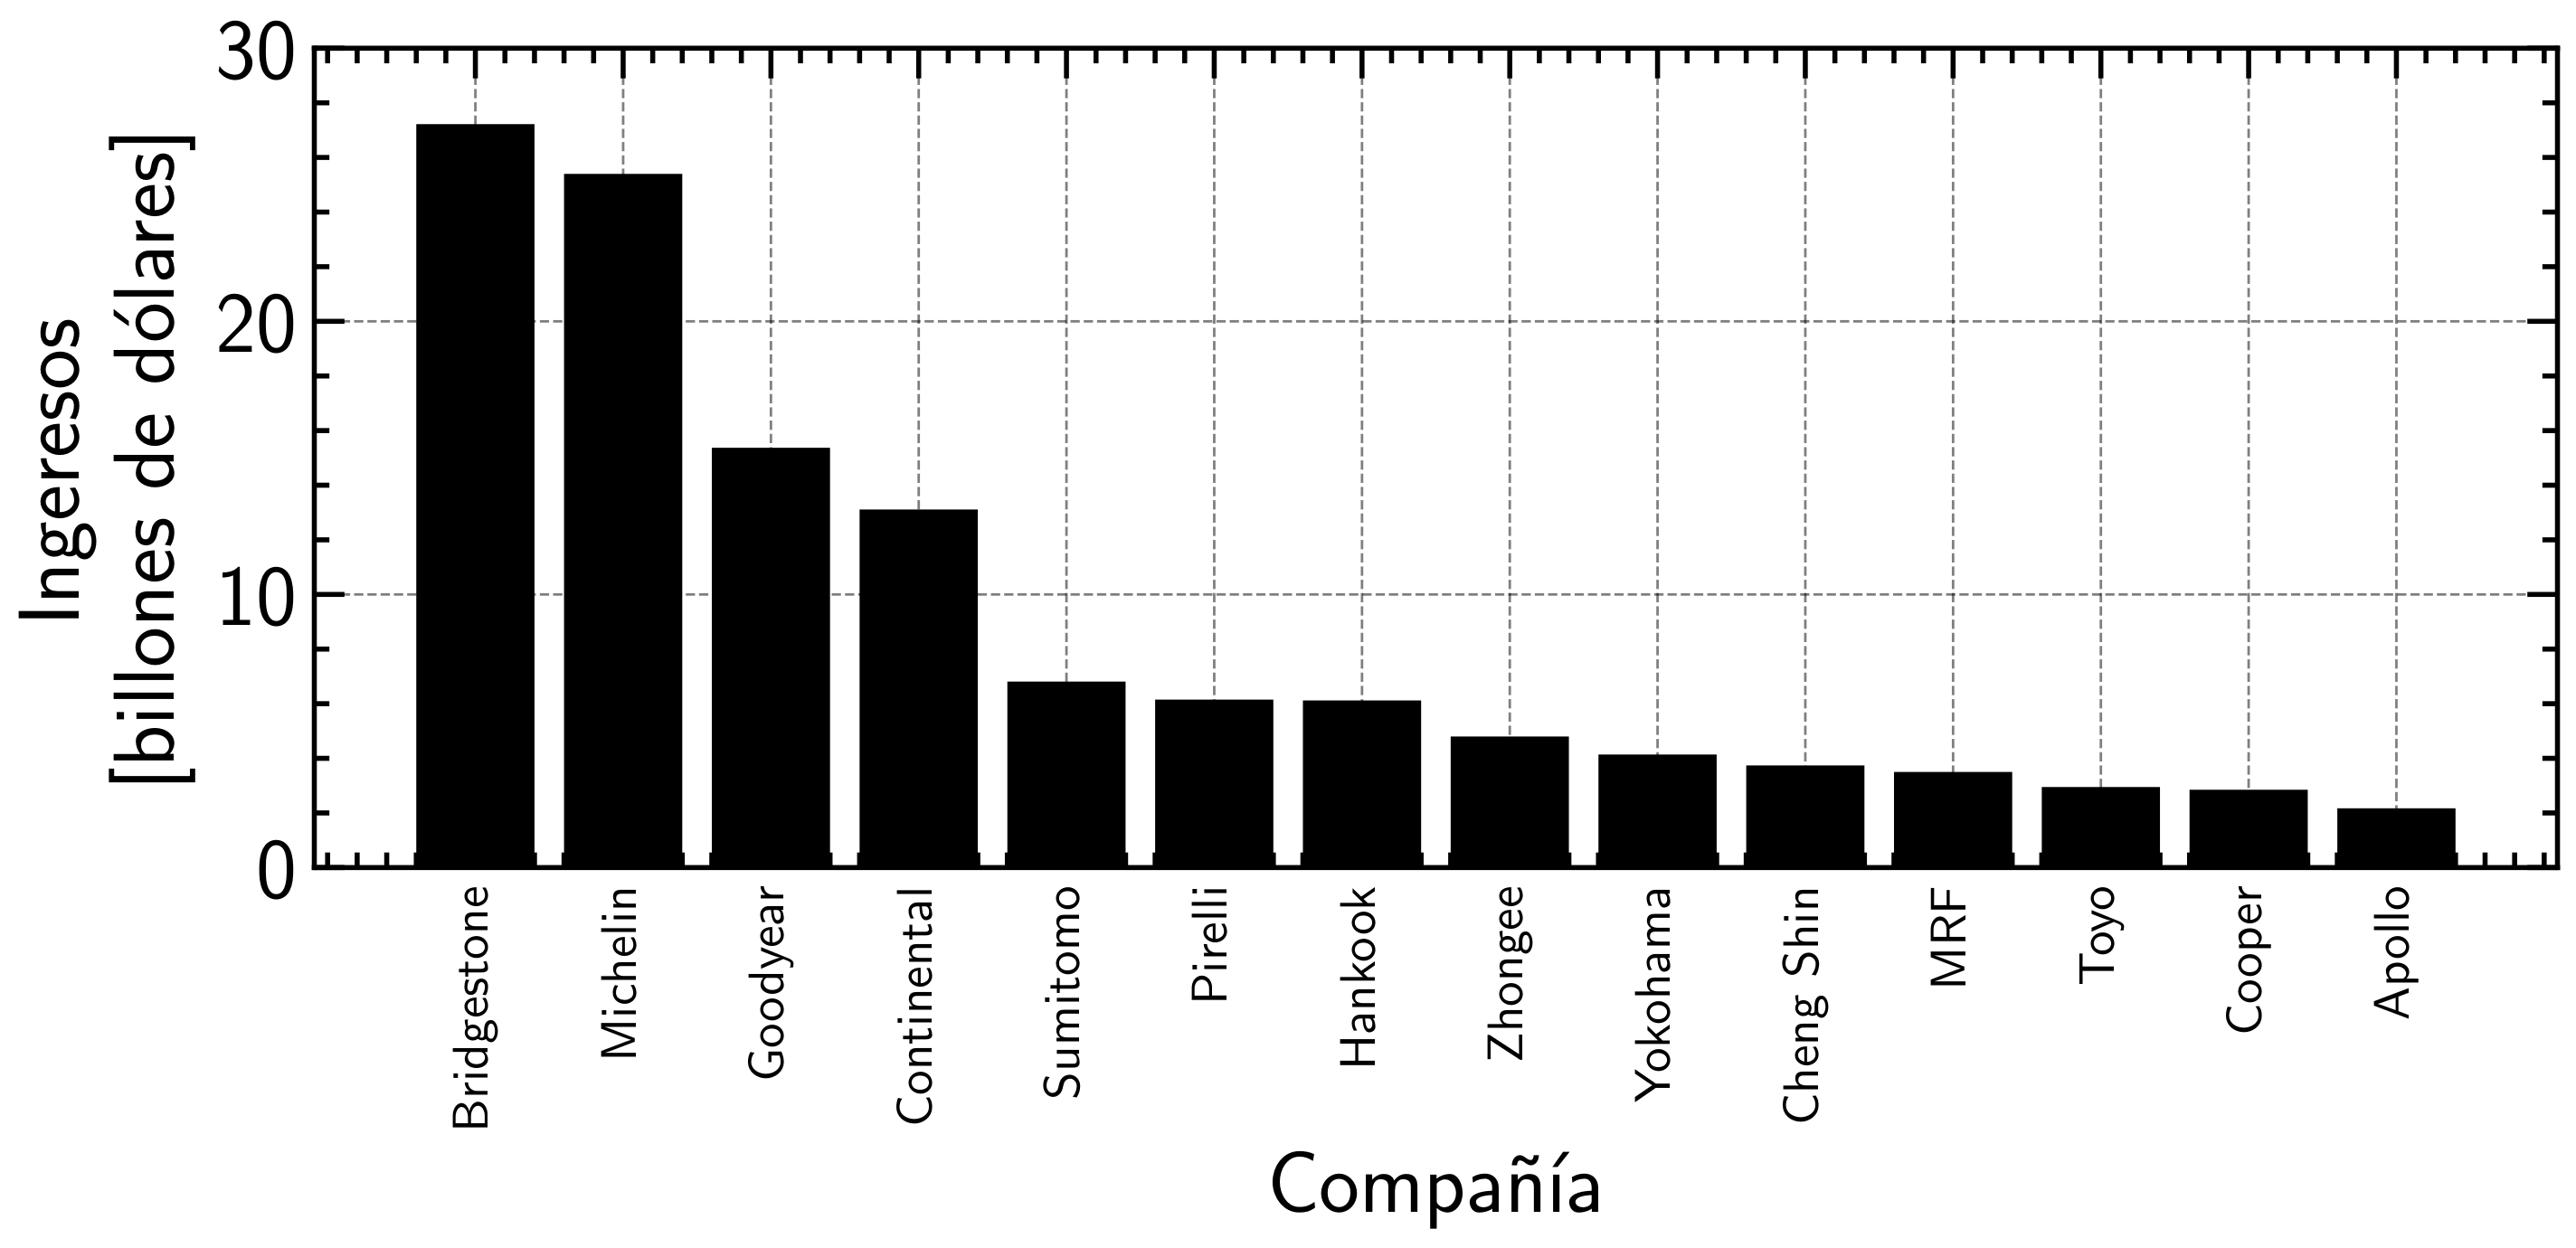
\includegraphics[width=\textwidth]{fig/1_brand.revenue.PNG}
	\end{center}
	\caption{Ingresos de los fabricantes de neumáticos más relevantes en 2019.}
	\label{fig:1_brand_revenue}
\end{figure}

La elevada competitividad característica del mercado,
sumada a la emergente comercialización de producto asiático,
incentiva a las establecidas multinacionales, a tomar un enfoque innovativo,
con la intención de mantener su liderazgo \citep{chicu2020current}.
El esfuerzo invertido en innovación,
por una parte, intenta alcanzar sus objetivos
mediante el rediseño y la mejora del producto.
Mientras que por la otra,
Trata de optimizar sus procesos y reducir desperdicios,
mediante la automatización y el uso inteligente de los recursos disponibles.

A la hora de implementar mejoras, ya sea a un producto o a un proceso,
la monitorización de los resultados y del cambio percibido se vuelve esencial.
El producto o proceso experimental debe satisfacer las expectativas del cliente,y a su vez, cumplimentar la legislación vigente,
como los estándares de calidad y medio ambiente.
La monitorización de estas mejoras implica un coste elevado,
a nivel temporal y económico, ya que estas deben ser puestas a prueba.
En el caso del producto, su industrialización,
supone reservar recursos que podrían ser destinados a la producción regular.
Desde la materia prima utilizada
en la elaboración de estos productos experimentales,
transitando por cada maquina ocupada para transformarlo,
hasta llegar a el laboratorio de calidad,
donde se realizan ensayos para otorgar feedback a el nuevo proceso.

El laboratorio de Calidad del Producto (LCP),
es el encargado de llevar a cabo los ensayos relevantes
para asegurar la conformidad de la producción.
A diario se cerciora de que los neumáticos manufacturados dentro de la planta
cumpla con los estándares de calidad definidos por la compañía.
El laboratorio logra asegurar la calidad del producto,
mediante un control estadístico de las muestras
elegidas al azar por cada gamma de producto.
Paralelamente, una fracción de los recursos disponibles,
es demandada por los proyectos de industrialización.
Obligando al departamento a equilibrar ambas necesidades.

En un entorno con recursos limitados,
donde la demanda no cesa de incrementar,
es cuestión de tiempo que los recursos se agoten
y la capacidad de el laboratorio se vea paralizada.
Para hacer frente a esta situación,
y poder mantener el esencial ritmo
marcado por los estándares de control de calidad e industrialización,
debe realizarse un escalado de los recursos del LCP.
A fin de que esta expansión, de este sistema complejo,
sea realizada de la manera optima,
debe realizarse un estudio de el impacto
de las inversiones que podrían realizarse, en la capacidad del LCP.
Para realizar esta tarea,
se ha optado por diseñar una Simulación de Eventos Discretos (DES)
que prevea los posibles futuros escenarios,
al cambiar algunas de las variables independientes de entrada.

El autor de este trabajo, se ha decantado por este método,
debido a la capacidad que ha demostrado
a la hora de resolver problemas de optimización en sistemas estocásticos.
Como menciona el autor \citep{allen2011introduction},
su versatilidad ha sido demostrada en numerosos ámbitos,como
aplicaciones militares,
sistemas sanitarios,
problemas logísticos
y optimización de procesos de manufacturación.

\subsection{OBJETIVOS}\label{sec_obj}
El objetivo principal de este trabajo
es proveer a la planta hipotética de cubiertas
con la información necesaria para la optima expansión del LCP.
Este trabajo se limitara a analizar los distintos escenarios investigados,
ofreciendo métricas e información cualitativa
sobre las distintas posibilidades,
para finalmente decantarse por la mejor opción.

Para lograr el objetivo final se deberán completar los siguientes subobjetivos:

\begin{itemize}
	\item Modelar los procesos del LCP
		de acuerdo a los fundamentos de una DES,
		obteniendo un modelo ajustado a la realidad.
	\item Definir las variables independientes del proceso,
		que posteriormente serán usadas en la simulación.
	\item Estimar el tiempo de ciclo de cada proceso,
		a través de la asignación de
		distribuciones ajustadas a cada subproceso.
	\item Definir las variables dependientes
		que otorgara el sistema a la salida.
	\item Desarrollar un programa de simulación en el entorno de Python
		mediante el uso de la librería Simpy.
		Dicha simulación, sera capaz de emular
		los distintos escenarios propuestos durante el desarrollo.
	\item Proponer una alternativa de la distribución de los recursos actuales
		para asegurar la capacidad del LCP cuando en el futuro aumente la
		demanda de ensayos.
\end{itemize}
